\section{3D-LIP Model with Heading Angles}\label{sec:lip}
If the full dynamic model of the humanoid is used to simulate its motion, it becomes computationally impossible to perform joint path and gait planning, due to its high dimensionality and non-linearity. Therefore, a simplifying model must be used. For this scope Peng et al. introduced the ``3D-LIP Model with Heading Angle'', which describes the discrete dynamics of the Center of Mass (CoM) similarly to the one of an inverted pendulum in three dimensions.

\subsection{Local Robot Reference Frame}
The state $\mathbf{x}$ and the input $\mathbf{u}$ of the dynamic model are defined as:
$$ \mathbf{x} := \left( p_x,\; v_x,\; p_y,\; v_y,\; \theta \right)^T \in \mathcal{X} \subset \mathbb{R}^5 , $$
$$ \mathbf{u} := \left( f_x,\; f_y,\; \omega \right)^T \in \mathcal{U} \subset \mathbb{R}^3 , $$

where $(p_x, v_x)$ are the CoM position and translational velocity along the $x$-axis, $f_x$ is the $x$-coordinate of the stance foot position, $\theta$ and $\omega$ are the humanoid's orientation and turning rate, respectively. $\mathcal{X}$ is the set of the allowed states, while $\mathcal{U}$ is the set of the admissible inputs.\\
Both the state and the input are expressed in the robot's local coordinates, which are time-related. This means that $(p_{x_k}, p_{y_k})$ represents the position of the CoM at simulation time step $k$ in the reference frame ($RF_k$) that originates from $(p_{x_{k-1}}, p_{y_{k-1}})$, and is rotated by an angle $\theta_k$ around the $z$-axis with respect to $RF_{k-1}$. The relation between the vectors in different reference frames is represented in Figure \ref{fig:loc_to_glob_tfm}.
The reference frame at time step 0 is considered the ``inertial'' or ``global'' frame. A transformation between the inertial and moving frames is necessary to obtain the position of the humanoid in the global map and to deal with obstacles.\\
These transformations are defined by the following matrix:
\begin{align}
    \mathbf{T}_k = 
    \begin{pmatrix}
        \mathbf{R}_k & \mathbf{t} \\[1ex]
        \ \mathbf{0} & 1
    \end{pmatrix}
    =
    \begin{pmatrix}
        \cos\theta_{k,\, \text{glob}} & -\sin\theta_{k,\, \text{glob}} & p_{x,\,k-1,\,\text{glob}} \\
        \sin\theta_{k,\, \text{glob}} & \cos\theta_{k,\, \text{glob}} &  p_{y,\,k-1,\,\text{glob}} \\
        0 & 0 & 1
    \end{pmatrix},
\end{align}
Starting from this, we transform the local vectors to the \textit{global reference frame} as follows:
\begin{align}
    \begin{pmatrix} 
        f_{x,\,k,\,\text{glob} } \\
        f_{y,\,k,\,\text{glob}} \\ 
        1 
    \end{pmatrix} = \; 
    \mathbf{T}_k \;
    \begin{pmatrix}
        f_{x,\,k,\,\text{loc} } \\
         f_{y,\,k,\,\text{loc}} \\
          1
    \end{pmatrix},\qquad \qquad
    \begin{pmatrix}
        p_{x,\,k,\,\text{glob} } \\
        p_{y,\,k,\,\text{glob}} \\[1ex]
        1
    \end{pmatrix}
    = \mathbf{T}_k \;
    \begin{pmatrix}
        p_{x,\,k,\,\text{loc} } \\
        p_{y,\,k,\,\text{loc}} \\[1ex]
        1
    \end{pmatrix},
\end{align}

\begin{align}
    \begin{pmatrix}
        v_{x,\,k,\,\text{glob} } \\[1ex]
        v_{y,\,k,\,\text{glob}}
    \end{pmatrix}
    = \mathbf{R}_k 
    \begin{pmatrix}
        v_{x,\,k,\,\text{loc} } \\[1ex]
        v_{y,\,k,\,\text{loc}}
    \end{pmatrix}
    =
    \begin{pmatrix}
        \cos\theta_{k,\, \text{glob}} & -\sin\theta_{k,\, \text{glob}} \\[1ex]
        \sin\theta_{k,\, \text{glob}} & \cos\theta_{k,\, \text{glob}}
    \end{pmatrix}
    \begin{pmatrix}
        v_{x,\,k,\,\text{loc} } \\[1ex]
        v_{y,\,k,\,\text{loc}}
    \end{pmatrix},
\end{align}
The positional vectors are roto-translated using a homogeneous matrix $ \mathbf{T}_k \in \mathbb{R}^{3\times3}$, while the velocity vectors are only rotated around the z-axis (indeed, a translation would change their magnitude) using a rotation matrix $\mathbf{R}_k \in \mathbb{R}^{2\times2}$.\\
The global robot's orientation is obtained by summing the latest local variation to the previous global angle, and the angular velocity does not need to be transformed because it is along the $z$-axis, which is fixed. Formally, they are defined as:
\begin{equation}
    \theta_{k+1, \text{glob}} \;=\; \theta_{k, \text{glob}} \,+\, \theta_{k+1, \text{loc}},
    \qquad
    \omega_{\text{glob}} \;=\; \omega_{\text{loc}}.
\end{equation}

An example of change of coordinates between the global and the local frame is illustrated in Figure \ref{fig:loc_to_glob_tfm}.

\todo[inline]{
    for simplicity, we used kept computations in local coordinates becuase the constraints are defined in local coordinates in original paper
}

\begin{figure}[h]
    \centering
    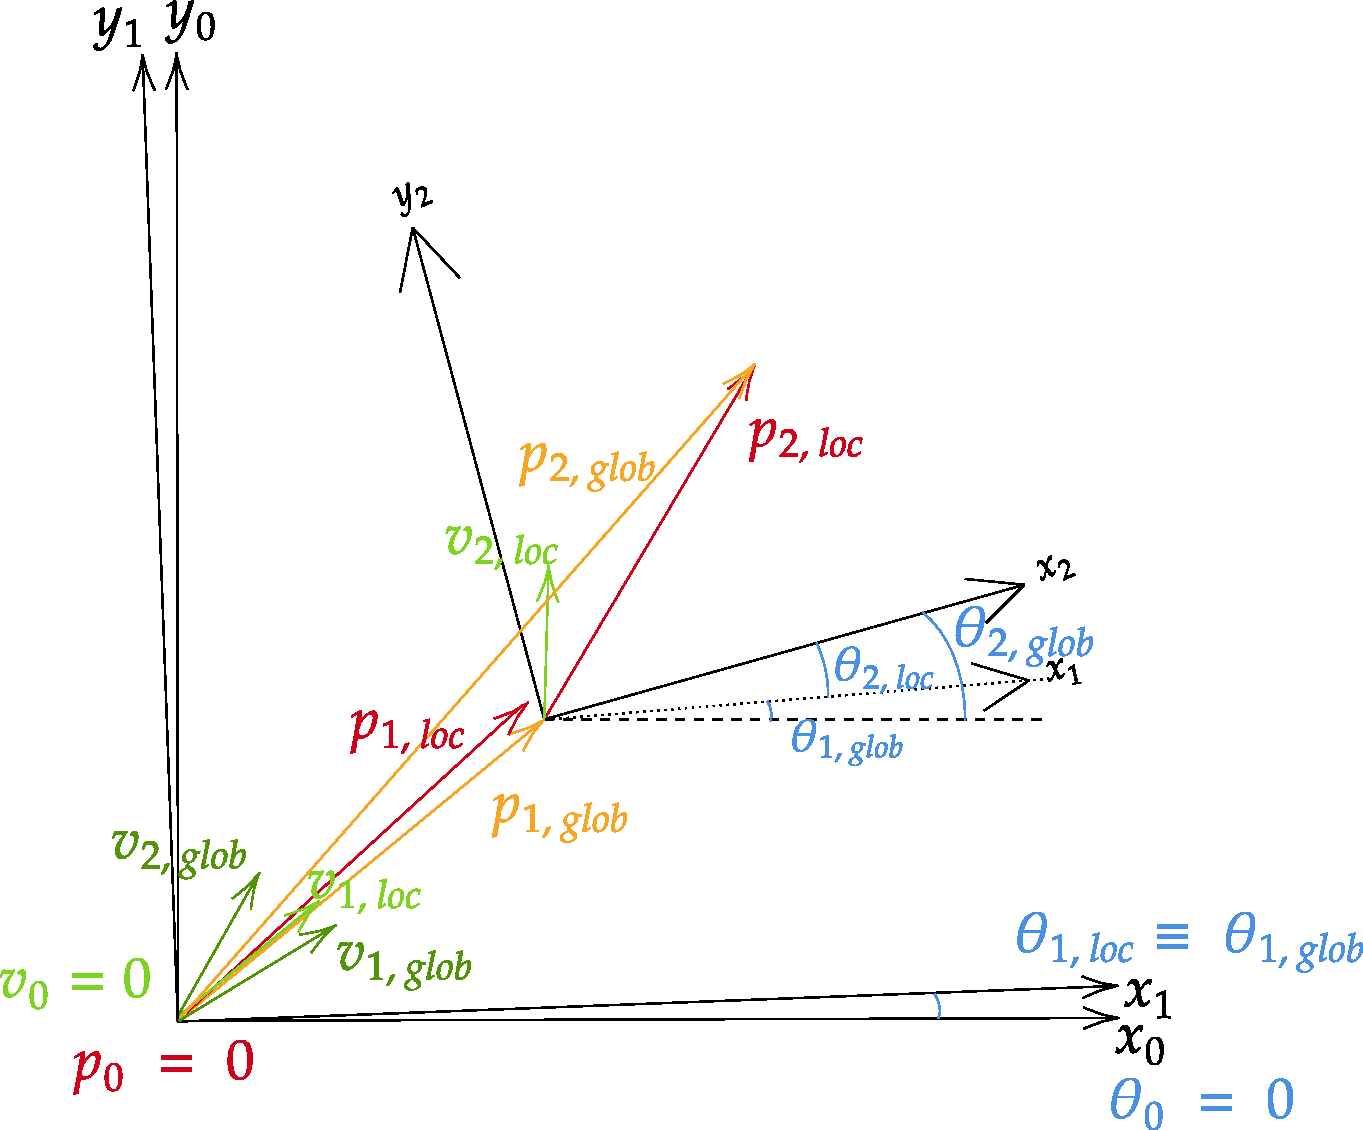
\includegraphics[width=0.75\linewidth]{figures/LIP/loc_to_glob_tfm2.pdf}
    \caption{An example of the evolution of the 3D-LIP model's state, highlighting the relationship between local and global coordinates. The initial state is $\mathbf{0}$ and the RF $(x_0,\, y_0)$ is the inertial frame. The local RF translates and rotates with the simulation time $k$: the position of $RF_2$ $(x_2,\, y_2)$ has its origin in $p_{1, \text{glob}}$, while its orientation is given by $\theta_{2, glob}$. The pose of the successive frames is computed analogously.}
    \label{fig:loc_to_glob_tfm}
\end{figure}

\subsection{Model Definition}
The Linear Inverted Pendulum formulation assumes that, the height $H$ of the CoM is constant during the motion.
According to \cite{peng_main_paper}, we can express the CoM acceleration as:
\begin{align}
    \begin{cases}
        \dot{v}_{x} = \dfrac{g}{H}(p_{x} - f_{x})
        \\[1ex]
        \dot{v}_{y} = \dfrac{g}{H}(p_{y} - f_{y})
    \end{cases},
\end{align}

with $g$ as the magnitude of the gravitational acceleration.
Based on this expression and the previously defined state $\mathbf{x}$ and input $\mathbf{u}$, we can define the 3D-LIP dynamic model in the continuous time space as:

\todo[inline]{add 0 dimension at subscript}

\begin{equation} \notag
\mathbf{\dot{x}}(t) = 
\begin{pmatrix}
    \dot{p}_{x}\\
    \dot{v}_{x}\\
    \dot{p}_{y}\\
    \dot{v}_{y}\\
    \dot{\theta}
\end{pmatrix} =
\mathbf{A_C} \, \mathbf{x}(t) + \mathbf{B_C} \, \mathbf{u}(t) =
\begin{pmatrix}
    \mathbf{A_h} & \mathbf{0} & \mathbf{0} \\
    \mathbf{0} & \mathbf{A_h} & \mathbf{0} \\
    \mathbf{0} & \mathbf{0} & \mathbf{0} \\
\end{pmatrix} \, \mathbf{x}(t) +
\begin{pmatrix}
    \mathbf{B_h} & \mathbf{0} & \mathbf{0} \\
    \mathbf{0} & \mathbf{B_h} & \mathbf{0} \\
    0 & 0 & 1\\
\end{pmatrix} \, \mathbf{u}(t),
\end{equation}
\begin{equation} \notag
\text{with:}\quad
\mathbf{A_h} \coloneq
\begin{pmatrix}
    0 & 1 \\
    \beta^2 & 0
\end{pmatrix},
\quad
\mathbf{B_h} \coloneq
\begin{pmatrix}
    0 \\
    -\beta^2
\end{pmatrix}, \quad
\beta \coloneqq \sqrt{\frac{g}{H}}.
\end{equation}

By further assuming that the duration of a single humanoid's step is fixed and equal to $T$, we can derive the closed-form step-to-step discrete dynamics of the 3D-LIP model:

\begin{equation}\label{eq:lip_dyanmics}
\mathbf{x}_{k+1} = \mathbf{A_L} \, \mathbf{x}_k + \mathbf{B_L} \, \mathbf{u}_k,
\end{equation}
with:
$$
\mathbf{A_L} \coloneqq 
\begin{pmatrix}
\mathbf{A_d} & \mathbf{0} & 0 \\
\mathbf{0} & \mathbf{A_d} & 0 \\
\mathbf{0} & \mathbf{0} & 1 \\
\end{pmatrix}, \qquad
\mathbf{B_L} \coloneqq 
\begin{pmatrix}
\mathbf{B_d} & \mathbf{0} & 0 \\
\mathbf{0} & \mathbf{B_d} & 0 \\
0 & 0 & T
\end{pmatrix},
$$
$$
\mathbf{A_d} \coloneqq 
\begin{pmatrix}
\cosh(\beta \, T) & \frac{\sinh(\beta \, T)}{\beta}  \\
\beta \, \sinh(\beta \, T) & \cosh(\beta \, T)
\end{pmatrix}, \qquad
\mathbf{B_d} \coloneqq 
\begin{pmatrix}
1 - \cosh(\beta \, T) \\
-\beta \, \sinh(\beta \, T)
\end{pmatrix}.
$$
\\
In the following chapter, these discrete dynamics will be used as the internal process representation of an MPC. Along with the constraints, they will grant that the found solution is meaningful to the humanoid motion.
